% !TEX root = ../../math_ia.tex
\subsection{Solid Cylinder}

For a solid, uniform cylinder of mass $M$, height $L$ and radius $R$, the process becomes more complicated due to the initial problem discussed in the background--different particles having different distances from the axis of rotation. Shapes such as those discussed above, although useful, are obviously elementary in their approach. More complicated/dense bodies such as solid cylinders are more routinely seen in physical applications, but have more nuance in their derivations as well. Consider a cylinder as shown in \cref{fig:rotating_solid_cylinder}.

% !TEX root = ../math_ia.tex
\begin{figure}[H]
  \centering
  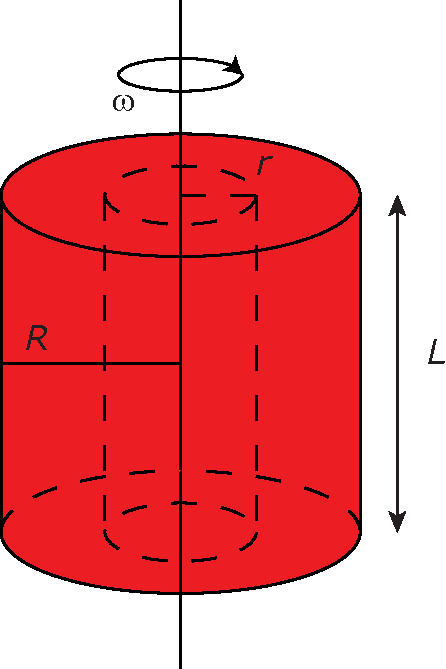
\includegraphics[width=0.25\linewidth]{fig/images/rotating_solid_cylinder.pdf}
  \caption{A solid cylinder rotating about a centered, perpendicular axis with a constant angular velocity $\omega$. A small shell of radius $r$ has also been depicted for visualization purposes}
  \label{fig:rotating_solid_cylinder}
\end{figure}

Assume the cylinder to have a constant density $\rho$, which leads to the determination:
\begin{gather*}
density = \frac{Mass}{Volume} = \frac{M}{V} \\
V = \pi R^2L \\
\rho = \frac{M}{\pi R^2L}\\
\end{gather*}
Consider the thin cylindrical shell formed from all the particles at a distance of $r$ from the axis of rotation, with a thickness $dr$ and a mass $dm$. Each of these shells' moment of inertia can then easily be transformed into an integral:
\begin{equation}
I = \int_0^M r^2dm
\end{equation}
as the perpendicular distance is represented by $r$ and the mass elements $dm$ are being summed over for the entire mass of the body. It is important to note, however, that $r$, $dm$ and $r^2$ are not constant in this integral, as they will depend on the specific shell. Thus, we must reduce from two variables down to one to solve for the moment of inertia.

The mass of shell can be represented as:
\begin{gather*}
dm = \rho dV \text{ (as mass} = \text{volume} \times \text{density)} \\
\end{gather*}
We can calculate $dV$ using the fact that the cylindrical shell has an infinitesimally small thickness. The shell can be cut and unfolded into a rectangular prism, with a width equal to the circumfrence of the shell, a thickness of $dr$, and a constant length of $L$:
\begin{gather*}
V = AL \\
dV = dAL \\
dV = 2\pi r dr L
\end{gather*}
Plugging this back into our formula for $dm$, we have:
\begin{gather*}
dm = \rho dV \\
dm = \rho 2\pi r dr L
\end{gather*}
As the distance of the shells from the axis of rotation ranges from $0$ to $R$, we must integrate over this interval while removing constants, resulting in:
\begin{gather*}
I = \int_0^R 2\pi\rho L r^3dr \\
I = 2\pi\rho L\int_0^R r^3dr \\
I = 2\pi\rho L\left[\frac{r^4}{4}\right]_0^R \\
I = 2\pi\rho\frac{R^4}{4}
\end{gather*}
Plugging in the initial value for $\rho$ calculated above, the resulting equation for the moment of inertia of a cylinder (using only the defined quantities of mass and total radius) is determined to be:
\begin{equation}
I_{\text{solid cylinder}} = \frac{1}{2}MR^2
\label{eq:final_moment_solid_cylinder}
\end{equation}

It is also important to note that this final formula for a cylinder is not dependent on the height $L$ of the cylinder, and thus the moment of inertia for a solid disk or cylindrical shape of any height can be calculated with this simple equation.